\documentclass[rep.tex]{subfiles}
\begin{document}

\chapter{Zadanie 16}
\label{zad16}
\section{Treść}
Zaprojektować filtr dolnoprzepustowy (FDP) o charakterystyce równomiernie falistej, rys.~\ref{fig:zad16:cheb},
dla następujących danych: $Z_0 = 50~\Omega$, $f_1 = 10^9~Hz$, $L_r = 0.2~dB$, $f_a = 1.43 \times 10^9~Hz$ i $L_a = 30~dB$.
Filtr zrealizować z odcinków linii współosiowej o średnicy przewodu zewnętrznego $D = 7~mm$, rys.16.2.
Obliczenia wykonać przy założeniu,
że impedancje charakterystyczne niskoomowych i wysokoomowych sekcji filtru są równe odpowiednio
$Z_l = 10~\Omega$ i $Z_h = 120~\Omega$.
Ponadto założyć, że niskoomowe sekcje filtru są odcinkami linii współosiowej wypełnionej dielektrykiem o $\epsilon_r = 2.05$ i $\mu_r = 1$.

\begin{figure}[!htbp]
  \centering
  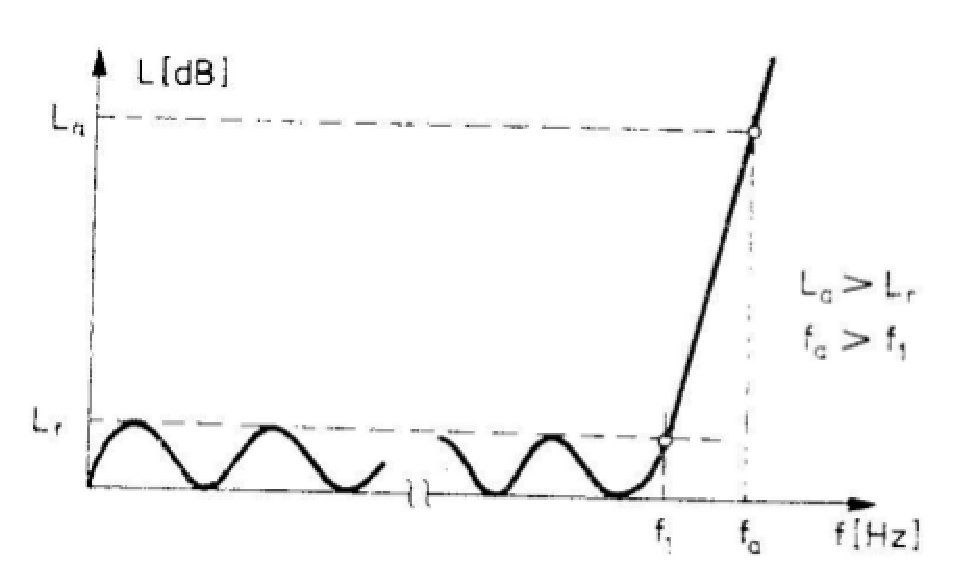
\includegraphics[scale=0.5]{fig/zad16/cheb}
  \caption{Charakterystyka projektowanego filtru}
  \label{fig:zad16:cheb}
\end{figure}

\begin{figure}[!htbp]
  \centering
  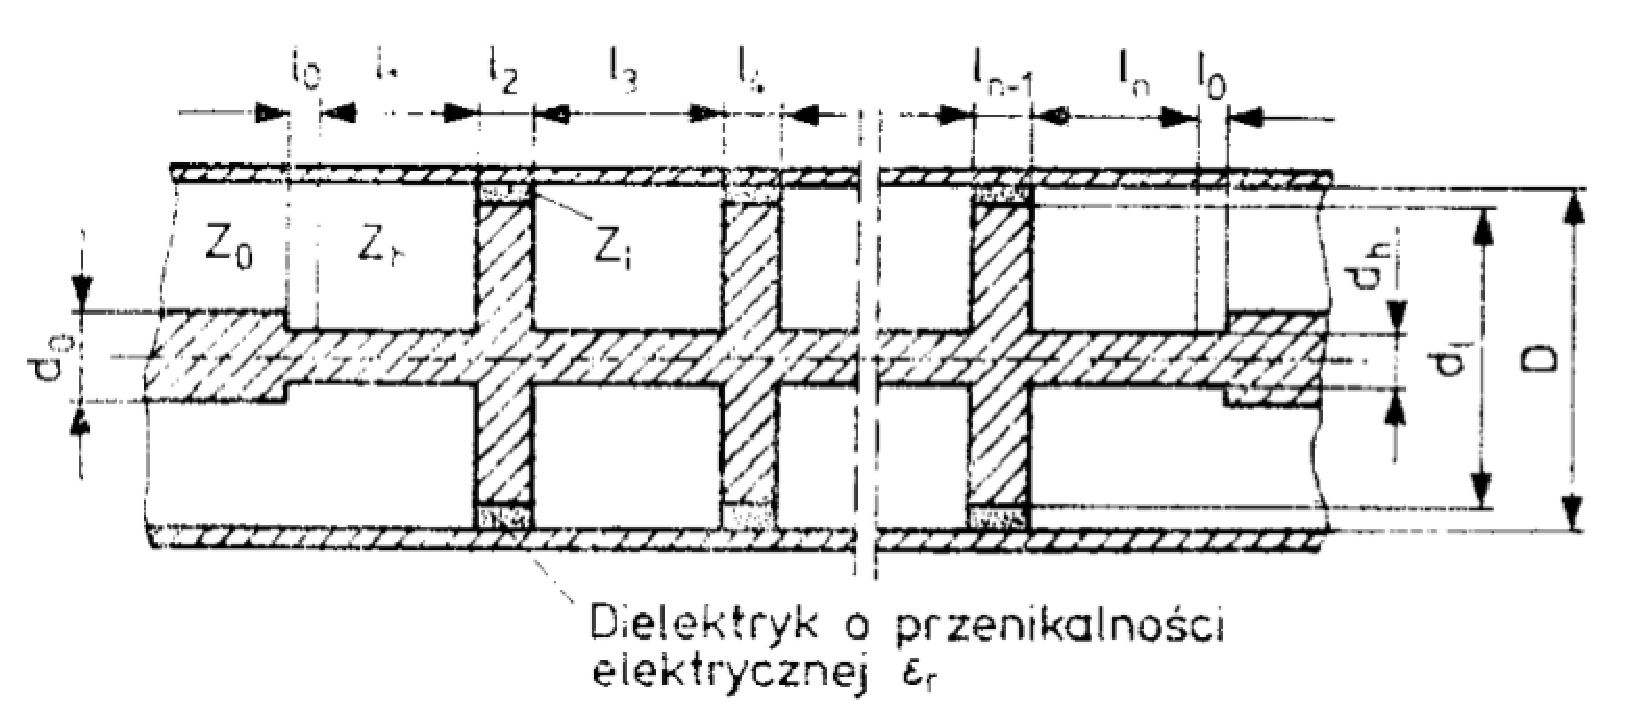
\includegraphics[scale=0.5]{fig/zad16/coax}
  \caption{Realizacja filtru przy użyciu linii współosiowej}
  \label{fig:zad16:coax}
\end{figure}

\section{Rozwiązanie}
W pierwszym kroku należy obliczyć minimalną ilość sekcji filtru:
\begin{align}
  n &\geq \frac{arch \sqrt{\frac{L_a' - 1}{L_r' - 1}}}{arch \Big(\frac{f_a}{f_1}\Big)} \\
  &= 7 \nonumber
\end{align}

Następnie należy obliczyć parametry filtru dolnoprzepustowego a na ich podstawie wartości elementów filtru o parametrach skupionych.
Wyniki tych obliczeń przedstawia tabela~\ref{tab:zad16:params}.
Długość $l_o$ stanowiąca poprawkę uwzględniającą pojemność~$C_{f0}$ wynosi $l_o = 2.60235408442~mm$.

\begin{table}
  \centering
  \caption{Parametry zaprojektowanego filtru}
  \label{tab:zad16:params}
  \begin{tabular}{l l l l l l l}
    \hline\hline
    i & g & L [nH] & C [pF] & l [mm] & $d_l$ [mm] & $d_h$ [mm]\\
    \hline
    0 & 1.0           &               &               &               & 3.04015838775 & 3.04015838775 \\
    1 & 1.37229535453 & 10.9203794528 & ---           & 28.6038828188 & ---           & 0.945831227808 \\
    2 & 1.37819320784 & ---           & 4.38692523125 & 6.05098425027 & 5.51288864551 & \\
    3 & 2.27568854642 & 18.109354055  & ---           & 57.3968306129 & ---           & 0.945831227808 \\
    4 & 1.50014664009 & ---           & 4.77511506265 & 6.02588104449 & 5.51288864551 &\\
    5 & 2.27568854642 & 18.109354055  & ---           & 57.3968306129 & ---           & 0.945831227808 \\
    6 & 1.37819320784 & ---           & 4.38692523125 & 6.05098425027 & 5.51288864551 &\\
    7 & 1.37229535453 & 10.9203794528 & ---           & 28.6038828188 & ---           & 0.945831227808 \\
    8 & 1.07602182984 & \\
    \hline\hline
  \end{tabular}
\end{table}
\end{document}
